\documentclass[10 pt,usenames,dvipsnames, oneside]{article}
\usepackage{../../../modelo-ensino-medio}



\begin{document}

\begin{center}
  \begin{minipage}[l]{3cm}

\includegraphics[width=2cm]{logo}    
\end{minipage}\hfill
\begin{minipage}[r]{.8\textwidth}
 {\Large \scshape Atividade: Ouvindo Funções Trigonométricas}  
\end{minipage}
\end{center}
\vspace{.2cm}

% \ifdefined\prof
% %Habilidades da BNCC
% % \begin{objetivos}
% % \item 
% % \end{objetivos}

% %Caixa do Para o Professor
% \begin{goals}
% %Objetivos específicos
% \begin{enumerate}

% \end{enumerate}

% \tcblower

% %Orientações e sugestões
% \begin{itemize}

% \end{itemize}
% \end{goals}

% \bigskip
% \begin{center}
% {\large \scshape Atividade}
% \end{center}
% \fi

No "\hyperref[trig-knowledge1]{Você Sabia: O Som e as Ondas Sonoras}"{},
você foi capaz de enxergar as ondas sonoras associadas a sons produzidos próximo ao seu aparelho celular. Nesta atividade faremos o caminho contrário: produziremos ondas sonoras no GeoGebra e iremos ouvi-las. Acesse o seguinte link para realizar a atividade: \url{https://www.geogebra.org/classic/sdx68rqp}

\begin{figure}[H]
\centering
\ifdefined\prof
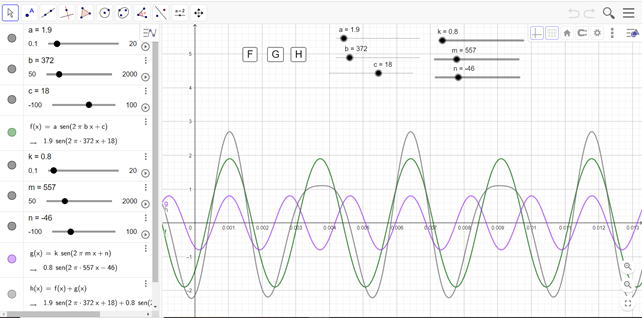
\includegraphics[width=.75\linewidth]{trigonometricas98}
\else
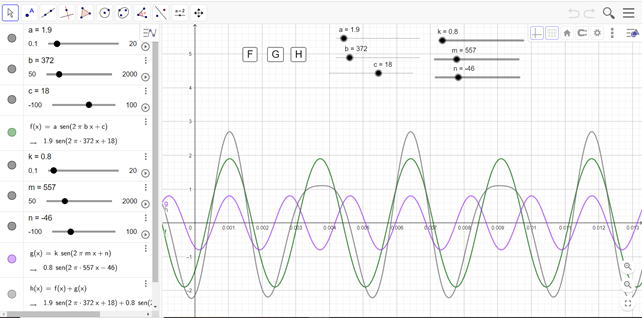
\includegraphics[width=.9\linewidth]{trigonometricas98}
\fi
\end{figure}

As ondas sonoras que você irá ouvir correspondem aos gráficos das seguintes funções:

\begin{align*}
F(x) &= a\cdot\sen(2\pi bx+c)\\
G(x) &= k\cdot\sen(2\pi mx+n) \text{ e}\\
H(x) &= F(x) + G(x)
\end{align*}

Repare que a função $H$ gera uma onda que é obtida combinando as ondas associadas a $F$ e $G$, visto que $H$ é dada pela soma de $F$ com $G$. Movimente os controles deslizantes $a$, $b$ e $c$ para alterar o formato da onda $F$, os controles $k$, $m$ e $n$ para alterar o formato da onda $G$ e qualquer um deles para alterar a onda $H$. Clique nos botões $F$, $G$ ou $H$ para ouvir o som associado à onda correspondente. Responda às perguntas:

\begin{enumerate}
\item Quais parâmetros estão associados à intensidade do som produzido?
\item Quais parâmetros estão associados à característica do som ser mais agudo ou mais grave?
\item Há algum parâmetro que ao ser movido não altera nenhuma característica do som? Qual(is)?
\item Há algum valor do parâmetro b para o qual você não consegue ouvir o som emitido pela onda $F$? Qual?
\end{enumerate}

\ifdefined\prof
\begin{solucao}

\begin{enumerate}
\item $a$ e $k$.
\item $b$ e $m$.
\item $c$ e $n$.
\item Abaixo de $10$ unidades já se vê uma dificuldade de ouvir o som da onda.
\end{enumerate}
\end{solucao}
\fi

\end{document}